\documentclass{standalone}

\usepackage{tikz,pgf} %and any other packages or tikzlibraries your picture needs

\begin{document}

%%%%%%%%%%%%%%%%%%%%%%%%%%%%%%%%%%%%%%%%%%%%%%%%%%%%%%%%%%%%%%%%%%%%%%%%%%%%%%%%
%COPY HERE
%%%%%%%%%%%%%%%%%%%%%%%%%%%%%%%%%%%%%%%%%%%%%%%%%%%%%%%%%%%%%%%%%%%%%%%%%%%%%%%%


\tikzset{every picture/.style={line width=0.75pt}} %set default line width to 0.75pt

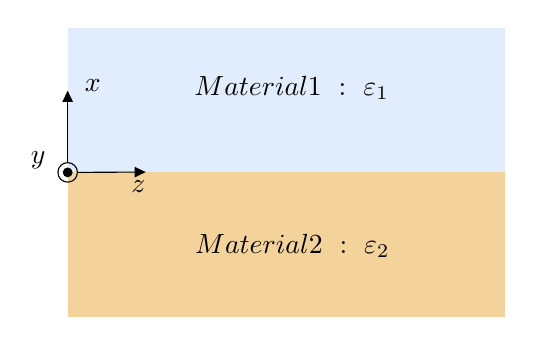
\begin{tikzpicture}[x=0.75pt,y=0.75pt,yscale=-1,xscale=1]
%uncomment if require: \path (0,300); %set diagram left start at 0, and has height of 300

%Shape: Rectangle [id:dp6791714378906519]
\draw  [draw opacity=0][fill={rgb, 255:red, 244; green, 210; blue, 155 }  ,fill opacity=1 ] (169.4,180.75) -- (380.2,180.75) -- (380.2,250.2) -- (169.4,250.2) -- cycle ;
%Shape: Rectangle [id:dp6526245353151652]
\draw  [draw opacity=0][fill={rgb, 255:red, 225; green, 237; blue, 252 }  ,fill opacity=1 ] (169.4,111.3) -- (380.2,111.3) -- (380.2,180.75) -- (169.4,180.75) -- cycle ;

%Shape: Circle [id:dp7413830003191302]
\draw   (164.7,180.75) .. controls (164.7,178.15) and (166.8,176.05) .. (169.4,176.05) .. controls (172,176.05) and (174.1,178.15) .. (174.1,180.75) .. controls (174.1,183.35) and (172,185.45) .. (169.4,185.45) .. controls (166.8,185.45) and (164.7,183.35) .. (164.7,180.75) -- cycle ;
%Shape: Circle [id:dp4002778696808824]
\draw  [fill={rgb, 255:red, 0; green, 0; blue, 0 }  ,fill opacity=1 ] (167.33,180.75) .. controls (167.33,179.6) and (168.25,178.68) .. (169.4,178.68) .. controls (170.55,178.68) and (171.48,179.6) .. (171.48,180.75) .. controls (171.48,181.9) and (170.55,182.83) .. (169.4,182.83) .. controls (168.25,182.83) and (167.33,181.9) .. (167.33,180.75) -- cycle ;
%Straight Lines [id:da47703583616511813]
\draw    (174.1,180.75) -- (204,180.61) ;
\draw [shift={(207,180.6)}, rotate = 539.74] [fill={rgb, 255:red, 0; green, 0; blue, 0 }  ][line width=0.08]  [draw opacity=0] (5.36,-2.57) -- (0,0) -- (5.36,2.57) -- cycle    ;
%Straight Lines [id:da5456358901162446]
\draw    (169.4,176.05) -- (169.4,144.4) ;
\draw [shift={(169.4,141.4)}, rotate = 450] [fill={rgb, 255:red, 0; green, 0; blue, 0 }  ][line width=0.08]  [draw opacity=0] (5.36,-2.57) -- (0,0) -- (5.36,2.57) -- cycle    ;


% Text Node
\draw (229.6,209.4) node [anchor=north west][inner sep=0.75pt]    {$Material2\ :\ \varepsilon _{2}$};
% Text Node
\draw (229.2,133) node [anchor=north west][inner sep=0.75pt]    {$Material1\ :\ \varepsilon _{1}$};
% Text Node
\draw (176.4,134.8) node [anchor=north west][inner sep=0.75pt]    {$x$};
% Text Node
\draw (150.4,169.6) node [anchor=north west][inner sep=0.75pt]    {$y$};
% Text Node
\draw (198.8,183.6) node [anchor=north west][inner sep=0.75pt]    {$z$};


\end{tikzpicture}



%%%%%%%%%%%%%%%%%%%%%%%%%%%%%%%%%%%%%%%%%%%%%%%%%%%%%%%%%%%%%%%%%%%%%%%%%%%%%%%%
%COPY HERE
%%%%%%%%%%%%%%%%%%%%%%%%%%%%%%%%%%%%%%%%%%%%%%%%%%%%%%%%%%%%%%%%%%%%%%%%%%%%%%%%

\end{document}
